\documentclass{article}\usepackage[]{graphicx}\usepackage[table]{xcolor}
% maxwidth is the original width if it is less than linewidth
% otherwise use linewidth (to make sure the graphics do not exceed the margin)
\makeatletter
\def\maxwidth{ %
  \ifdim\Gin@nat@width>\linewidth
    \linewidth
  \else
    \Gin@nat@width
  \fi
}
\makeatother

\definecolor{fgcolor}{rgb}{0.345, 0.345, 0.345}
\newcommand{\hlnum}[1]{\textcolor[rgb]{0.686,0.059,0.569}{#1}}%
\newcommand{\hlstr}[1]{\textcolor[rgb]{0.192,0.494,0.8}{#1}}%
\newcommand{\hlcom}[1]{\textcolor[rgb]{0.678,0.584,0.686}{\textit{#1}}}%
\newcommand{\hlopt}[1]{\textcolor[rgb]{0,0,0}{#1}}%
\newcommand{\hlstd}[1]{\textcolor[rgb]{0.345,0.345,0.345}{#1}}%
\newcommand{\hlkwa}[1]{\textcolor[rgb]{0.161,0.373,0.58}{\textbf{#1}}}%
\newcommand{\hlkwb}[1]{\textcolor[rgb]{0.69,0.353,0.396}{#1}}%
\newcommand{\hlkwc}[1]{\textcolor[rgb]{0.333,0.667,0.333}{#1}}%
\newcommand{\hlkwd}[1]{\textcolor[rgb]{0.737,0.353,0.396}{\textbf{#1}}}%
\let\hlipl\hlkwb

\usepackage{framed}
\makeatletter
\newenvironment{kframe}{%
 \def\at@end@of@kframe{}%
 \ifinner\ifhmode%
  \def\at@end@of@kframe{\end{minipage}}%
  \begin{minipage}{\columnwidth}%
 \fi\fi%
 \def\FrameCommand##1{\hskip\@totalleftmargin \hskip-\fboxsep
 \colorbox{shadecolor}{##1}\hskip-\fboxsep
     % There is no \\@totalrightmargin, so:
     \hskip-\linewidth \hskip-\@totalleftmargin \hskip\columnwidth}%
 \MakeFramed {\advance\hsize-\width
   \@totalleftmargin\z@ \linewidth\hsize
   \@setminipage}}%
 {\par\unskip\endMakeFramed%
 \at@end@of@kframe}
\makeatother

\definecolor{shadecolor}{rgb}{.97, .97, .97}
\definecolor{messagecolor}{rgb}{0, 0, 0}
\definecolor{warningcolor}{rgb}{1, 0, 1}
\definecolor{errorcolor}{rgb}{1, 0, 0}
\newenvironment{knitrout}{}{} % an empty environment to be redefined in TeX

\usepackage{alltt}

\usepackage{lineno,hyperref}
\modulolinenumbers[5]


\usepackage[normalem]{ulem} % Allow strikethrough text
\usepackage{float}
\usepackage{booktabs}
\usepackage{fullpage}
\usepackage{graphicx}
\usepackage{amsmath,amssymb}

\usepackage{natbib}
\bibliographystyle{plain}

%%%%%%%%%%%%%%%%%%%%%%%

%%% Commenting %%%%%%%%%%%%%%%%%%%%%%%%%%%%%%%%%%%%%%%%%%%%%%%%%%%%%%%%%%%%%%%%%
% \usepackage[table,dvipsnames]{xcolor}
\newcommand{\mt}[1]{{\color{magenta} #1}}
\newcommand{\svp}[1]{{\color{teal} #1}}
\newcommand{\fix}[1]{{\color{orange} #1}}
%%%%%%%%%%%%%%%%%%%%%%%%%%%%%%%%%%%%%%%%%%%%%%%%%%%%%%%%%%%%%%%%%%%%%%%%%%%%%%%%










\title{A Convolutional Neural Network for Outsole Recognition\footnote{This work was partially funded by the Center for Statistics and Applications in Forensic Evidence (CSAFE) through Cooperative Agreement \#70NANB15H176 between NIST and Iowa State University, which includes activities carried out at Carnegie Mellon University, University of California Irvine, and University of Virginia.}}

%% Group authors per affiliation:
\author{Miranda Tilton and Susan Vanderplas}
% \address{Center for Statistics and Applications in Forensic Evidence, Iowa State University. 195 Durham Center, 613 Morill Rd., Ames, IA 50011}
\IfFileExists{upquote.sty}{\usepackage{upquote}}{}
\begin{document}
\maketitle
\begin{abstract}
Quantitative assessment of class characteristic frequency is a difficult problem, in part because there is currently no way to collect and efficiently process the quantity of data that would be required for such assessments without prohibitive amounts of human labor. In this paper, we discuss a computational method which complements a passive, unmanned scanning device that is currently under development. The automatic class characteristic recognition algorithm described in this paper has been developed with photographs of outsole images, and identifies high-level geometric features such as circles, stars, and quadrilaterals. These features are designed to mimic high-level features used by examiners to facilitate automatic processing of features without resorting to black-box feature sets commonly used in neural networks. The algorithm performs well on images with unambiguous shapes and moderate color contrast, though some systematic errors arise from the physical similarities of geometric shapes. Additional improvements may be realized by modifying the labeling scheme to reduce feature overlap and by preprocessing the images to improve contrast. This new approach represents a significant step toward enabling the collection and application of population-level class characteristic data to support quantitative assessments of the value of class-characteristic based similarity assessments.
\end{abstract}
%
% \begin{keyword}
% Footwear; class characteristics; \mt{random match probability}; computer vision; neural networks
% \end{keyword}

% \end{frontmatter}

\linenumbers

\section{Introduction}\label{sec:Introduction}

Collection and use of footwear evidence varies heavily across jurisdictions within the United States, and, though it is more common for such analyses to be used in Europe, the U.K., and Israel, many of the same fundamental issues remain. It is often difficult to recover footwear evidence with sufficient detail to identify individualizing characteristics, either because of degradation or because the medium did not record the individualizing characteristics in sufficient detail to examine. It is also common for prints to be only partially recorded or recovered, which further compounds the difficulty of performing these types of analysis. As a result, the majority of footwear examinations in the United States reach conclusions regarding the correspondence of class characteristics rather than of individualizing characteristics \citep{smith_2011}. This tendency is also reflected in the SWGTREAD range of conclusions scale, which has two separate categories to indicate degrees of class characteristic based association out of a range of 7 conclusions\citep{SWGTREAD2013}. Currently, the guidelines also caution against any statistical assessment because accurate data and models to support statistical calculations do not exist. However, if it were possible to collect a sufficiently large quantity of footwear impression data from a local population, it would be helpful to be able to calculate the frequency of shoes in the population that have similar class characteristics to a given shoe or print in order to characterize the determinative value of that particular piece of evidence. Note that this question is distinct from make and model determination since many shoes of different makes and models can still have similar tread patterns on the class characteristic level.

Statistically, the coincidental (or random) match probability is estimated by sampling a large number of shoes from a given population and calculating the observed proportion of shoes in the sample whose tread patterns are similar to the given print. The primary obstacle to coincidental match probability calculation, then, is one of data collection and annotation. The (limited) number of population class-characteristic studies \citep{parent_sandy_significance_nodate,benedict_geographical_2014} demonstrate the effort required to collect, process, and analyze even a moderate amount of data manually. However, technological innovations over the past decade have automated previously manual tasks such as license plate reading, tracking individuals on video feeds, and other complex tasks. In these comparable situations, two separate but related technological innovations were required: inexpensive and automatic data collection hardware (e.g. via CCTV or video cameras), and automatic, accurate data processing software. We are in the process of developing a low-profile scanner which, when embedded in a pedestrian area, passively collects images of shoe treads (a prototype is shown in \autoref{fig:prototype-scanner}). In parallel, however, it is necessary to develop software which can process the data from a similarly oriented scanner to generate features which are used to make class characteristic comparisons. Through the combination of hardware and software, we hope to enable the collection of population-level footwear data which will facilitate quantitative assessment of class characteristic frequency to support examiner evaluation.


\begin{figure}
\centering
\setlength\tabcolsep{1mm}
\begin{tabular}{cc}
\raisebox{-.5\height}{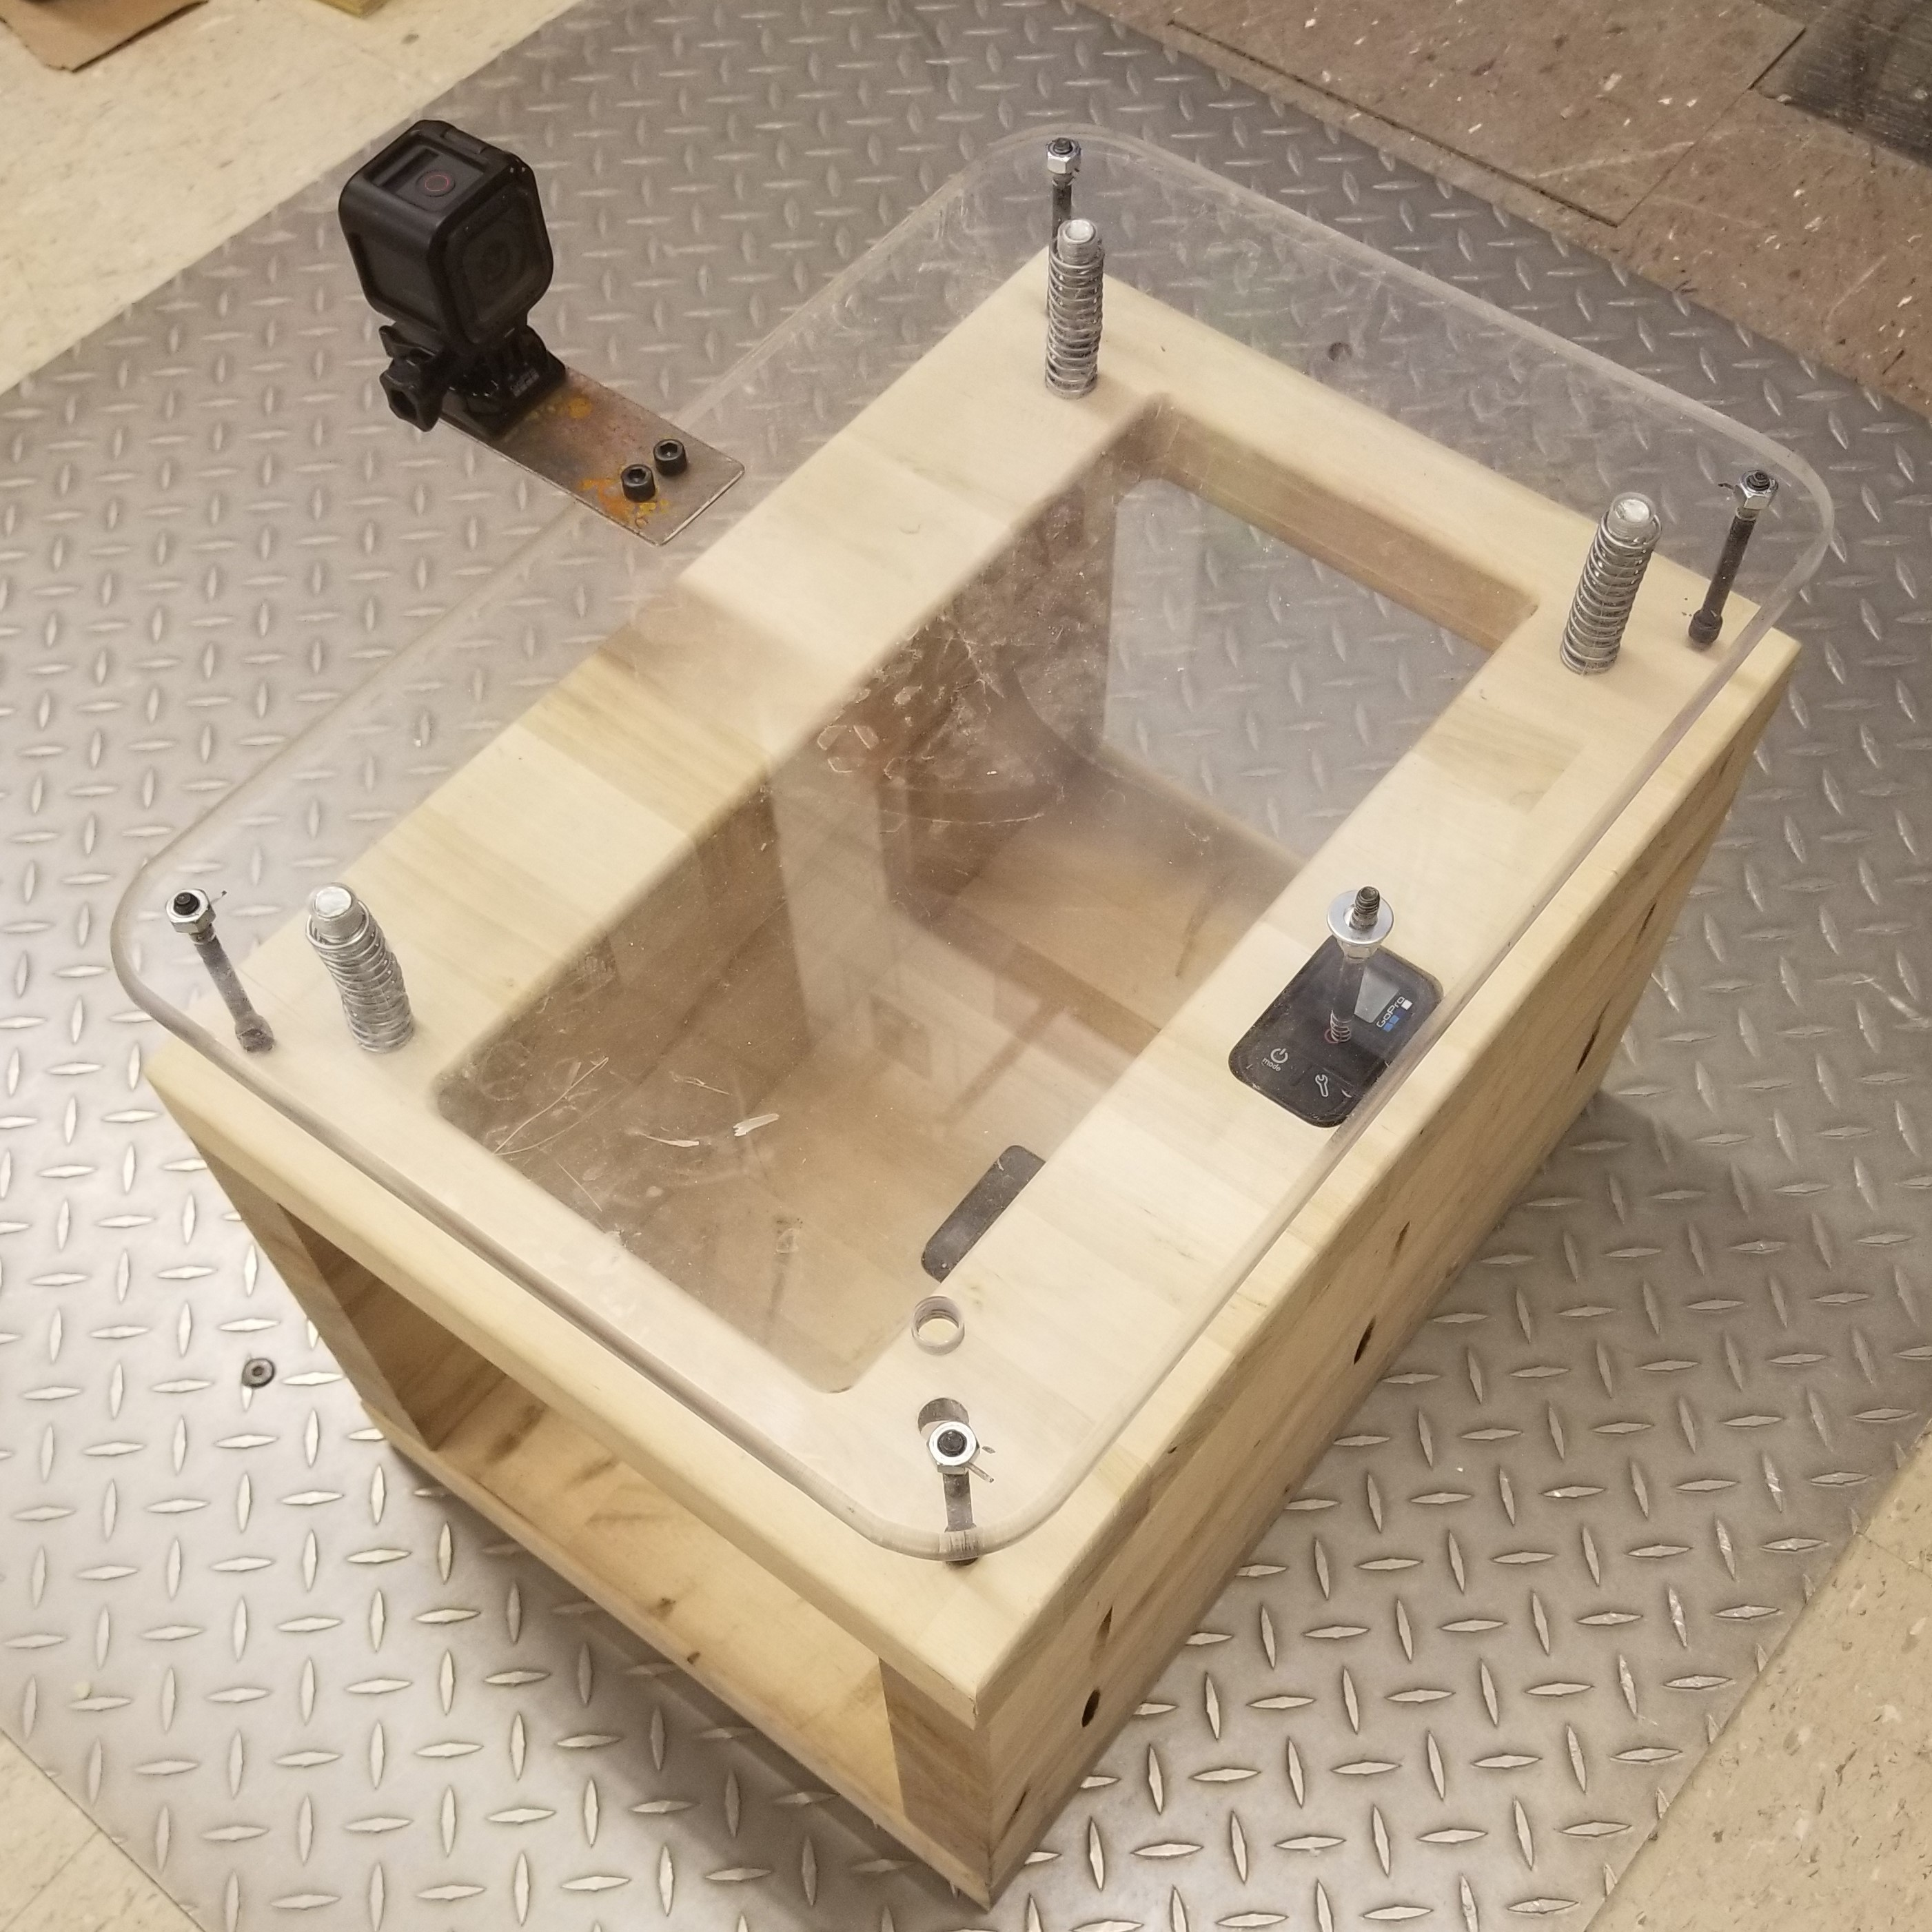
\includegraphics[width=.45\textwidth]{images/prototype/20200402_151639.jpg}} &
\raisebox{-.5\height}{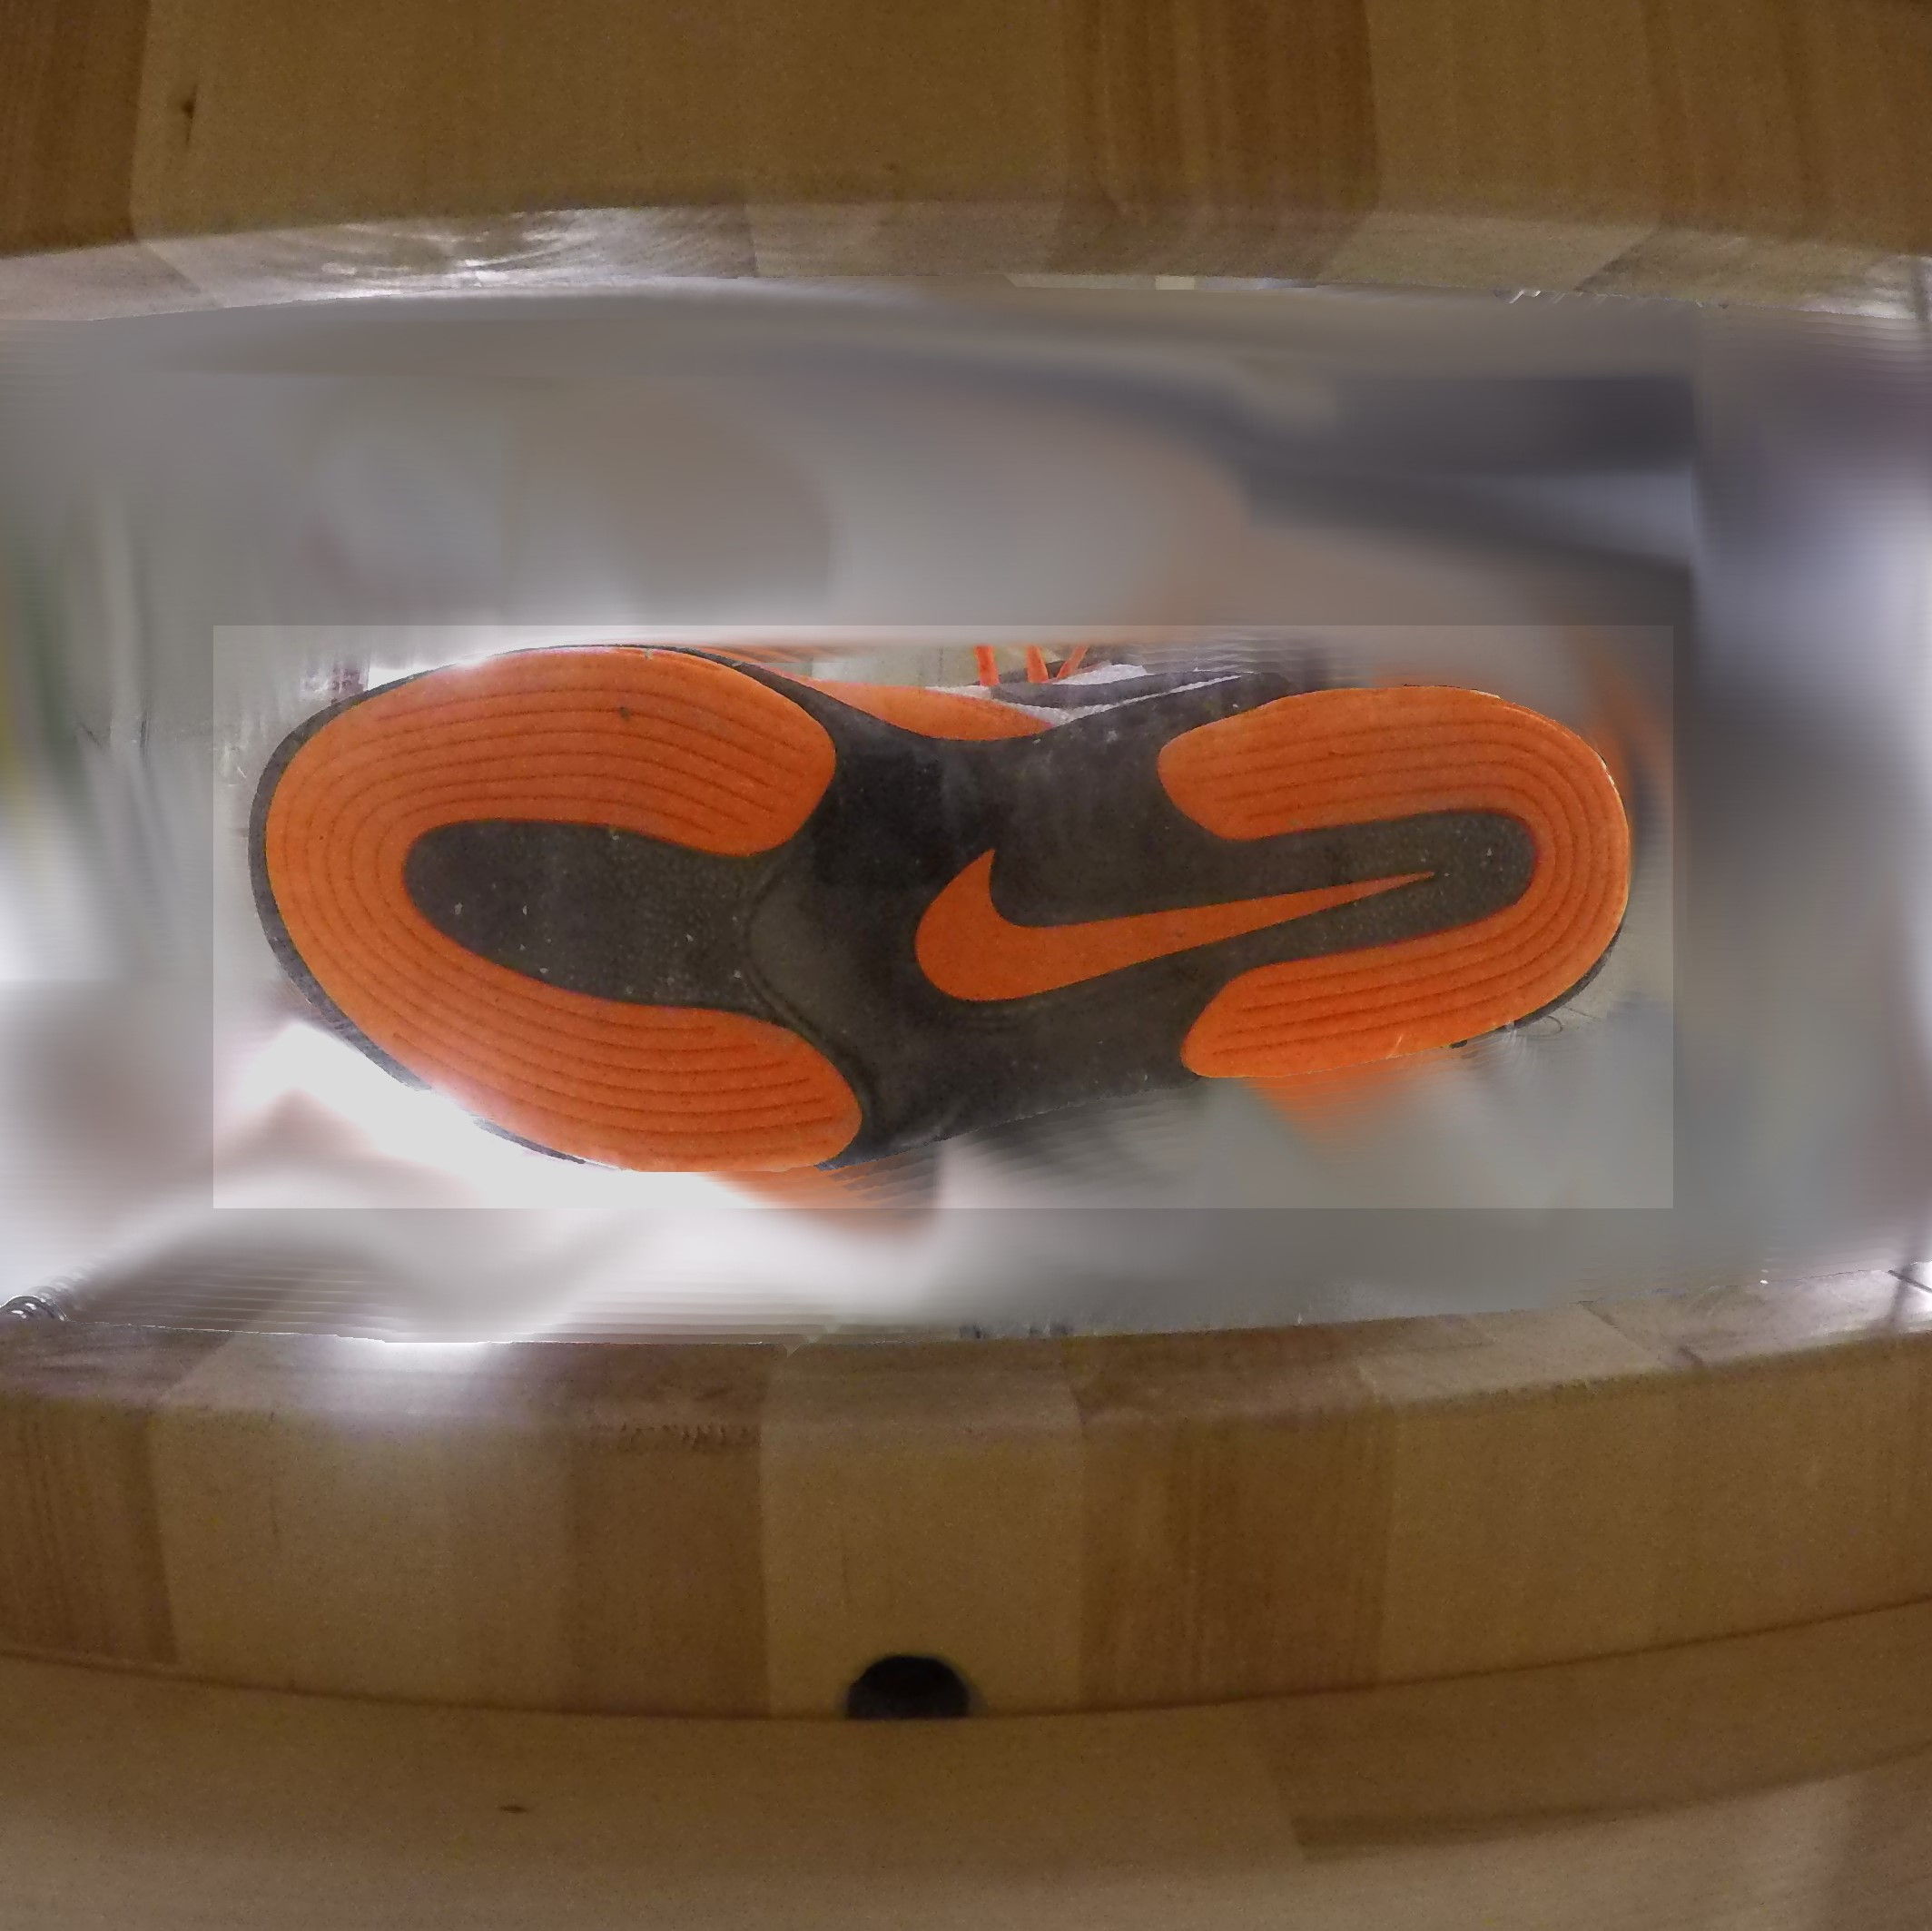
\includegraphics[width=.45\textwidth]{images/prototype/GOPR1231-blur-enhance_square.jpg}} \vspace{1mm}\\

\end{tabular}
\caption[Images of prototype scanner.]{Images of the prototype scanner for collecting a large number of outsole images.}\label{fig:prototype-scanner}
\end{figure}


\subsection{Image Analysis}

% From original intro:
Several attempts have been made to automatically identify features in both prints and shoe tread images, with low-level image analysis methods including fractal decomposition \citep{alexanderAutomaticClassificationRecognition1999}, scale-invariant feature recognition \citep{pavlouAutomaticExtractionClassification2006}, Fourier-Mellin transformation \citep{guehamAutomaticRecognitionShoeprints2008}, and other classical image analysis methods. Some of these low-level methods perform relatively well in good conditions \citep{luostarinenMeasuringAccuracyAutomatic2014a} but have degraded performance under conditions which are suboptimal, including those commonly found at crime scenes.

% From original intro:
In the wider field of computer vision, attention has turned to more robust methods for image recognition, such as convolutional neural networks (CNNs), which are capable of achieving near-human accuracy under even degraded image conditions \citep{krizhevskyImageNetClassificationDeep2012}. These networks are designed to mimic the process of human vision, and typically involve application of sets of filters, some of which mimic the filters used in the low-level techniques used in early automatic classification attempts. CNNs have been applied in footwear forensics, making use of more general neural networks optimized to detect objects found in natural scenes, such as trees, animals, buildings, and cars; the pre-trained network's features are then used to compare shoes or prints to determine how well they match \citep{kongCrossDomainImageMatching2019a,kongCrossDomainForensicShoeprint2017,zhangAdaptingConvolutionalNeural2017}. Neural network methods appear to be more successful than traditional image analysis techniques, but the features used for matching are not generally informative for humans, who typically classify shoes by patterns and spatial relationships \citep{davisIntelligenceApproachFootwear1981,grossVariabilitySignificanceClass2013}.


Although footwear impressions are more commonly used in practice for footwear analysis than outsole images, our early prototypes of a footwear scanner suggest that cameras are more robust than impression-based systems (e.g.  EverOS) for use in outdoor settings. As a result, in this paper describing an initial automated software system for class characteristic recognition, we use outsole images (such as those found on online retail sites) rather than impression-based training data. While we recognize that images from the scanner are likely to show some degradation compared to images found from online retailers, the fundamental features of the underlying machine learning models are similar. In this paper, we present a proof-of-concept model designed to identify class characteristics probabilistically, using labels similar to those used by examiners. We discuss the strengths and limitations of both the classification scheme and the neural-network based model, with important implications for future attempts to develop automatic high-level class characteristic recognition systems.


\section{Materials and Methods}

Images collected from a footwear scanner (as described in the previous section) would be stored in photographic form; as a result, we must use image analysis methods to create numerical features from the original visual record. There are a number of methods that may be employed to identify shapes and features in an image, such as Fourier-Mellin transforms, Hough transformations \citep{ballardGeneralizingHoughTransform1981} and other low-level feature extraction methods aimed at detecting specific shapes, such as edges, corners, blobs, or ridges \citep[Ch 15]{machineVision}. While these methods are useful in identifying these specific features at a low level, they only identify features on a very small scale; as a result, they cannot reliably identify large geometric shapes like those that may be found in a high resolution outsole image.

Convolutional neural networks (CNNs) are widely recognized as superior for novel image classification and feature detection. CNNs are a form of artificial neural network which make use of the image convolution operator used by many low-level feature extraction methods, with the additional ability to aggregate such features and meaningfully connect them to a pre-determined set of labels. CNNs have deep architectures that can be trained to identify complex patterns, but they are structurally similar to the architecture of the human visual system and output binary or probabilistic predictions for given labels that are readily interpretable. As CNNs make use of labeled training data, the predictions generated are for features which are similar to those identified by humans, resulting in models with greater face validity. Once a CNN is trained, it is relatively fast and easy to apply the model to new images and obtain classifications.

\paragraph{Transfer Learning}
Neural networks are composed of sets of layers; the early layers, which are called the model base, contain feature detectors, and the final layers make up the classifier, or model head, which connects meaningful features to classification labels (see \autoref{fig:VGG16-structure} for an example of the structure of a CNN). Each of these layers is composed of sets of weights and connections that are optimized during training. A relatively simple convolutional neural network which processes image data may contain more than 14 million parameters in the model base and an additional 120 million parameters in the model head; to train a model of this nature requires millions of labeled images and a significant amount of computational power. Assembling sufficient data to train a network from scratch is a gargantuan task; the process of \emph{transfer learning} is a natural solution to this common problem. Transfer learning leverages the modularity of neural networks, that is, that the model base that detects features can be separated from the classifier which produces predictions. Transfer learning approaches use the base of a model trained on more general image data and train a new model head or classifier using a smaller set of domain-specific labeled images\citep{oquabLearningTransferringMidlevel2014}. This allows CNNs to be applied to smaller datasets of several thousand images, reduces the amount of computational time required to fit the model, and provides boosted performance compared to training a new model from scratch \citep{yosinskiHowTransferableAre2014}. Transfer learning has been successfully applied in automatic classification of medical images \citep{shinDeepConvolutionalNeural2016} as well as in various applications of shoe forensics \citep{kongCrossDomainForensicShoeprint2017,kongCrossDomainImageMatching2019a,zhangAdaptingConvolutionalNeural2017}.

Many convolutional neural networks have been trained on a subset of images from an online image database called ImageNet \citep{dengImageNetLargeScaleHierarchical}. In particular, there is a standard set of images from ImageNet, consisting of 1.2 million images that span 1,000 categories, that is commonly used in computer vision tasks. CNNs trained on ImageNet are optimized for general human-like vision, that is, the ability to recognize a large set of different features simultaneously. As a result, the base of networks trained on these sets are often used for transfer learning, because the initial layers are broadly generalizable to a wide variety of more specific image labeling tasks. In the next section, we will introduce the pre-trained network VGG16, pictured in \autoref{fig:VGG16-structure}, and examine a selection of its filters (shown in \autoref{fig:vgg16layers}) that demonstrate the levels of detail in the initial layers of a model trained on generic data.


\begin{figure}
\centering
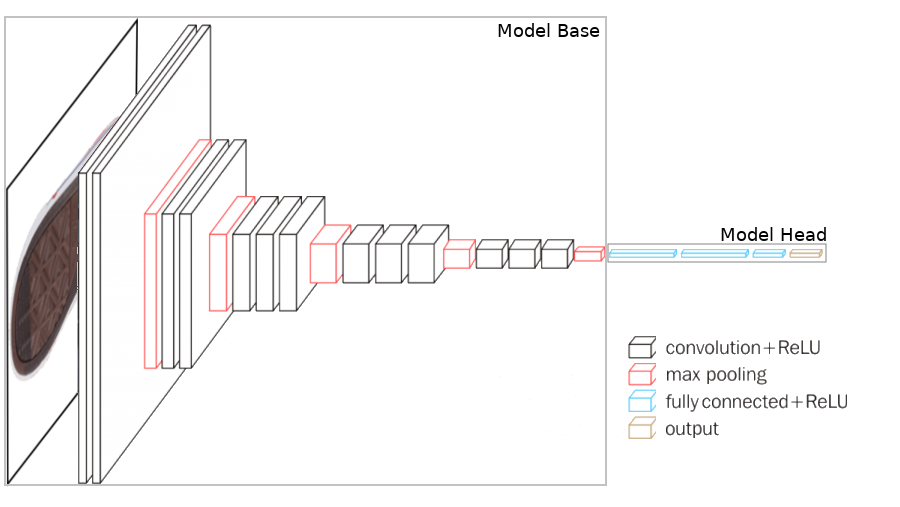
\includegraphics[width=\textwidth]{images/vgg16-shoe-nolabel}
\caption[VGG16 structure]{VGG16 consists of five convolutional blocks that make up the model base. Each convolutional block contains an increasing number of increasingly complex feature-detecting filters. After the convolutional blocks, the fully connected layers of the model head are used to make global connections between separate features.}\label{fig:VGG16-structure}
\end{figure}

\paragraph{VGG16}
Developed by Oxford's Visual Graphics Group, VGG16 is a CNN trained on ImageNet
\citep{krizhevskyImageNetClassificationDeep2012}. In contrast to other popular pre-trained networks, such as AlexNet or ResNet, VGG has a relatively simple structure that provides easier training and interpretability with very little sacrificed accuracy. The simplicity of this structure provides the ability to peer into the inner workings of the network for diagnostic purposes, providing a distinct advantage over more complicated network structures with slightly higher accuracy ratings. VGG16 is a common choice for transfer learning because of this structural simplicity; it has been used for detection of text in natural images \citep{zhongDeepTextUnifiedFramework2016}, medical imaging classification \citep{oquabLearningTransferringMidlevel2014}, classification of weld defects \citep{liuWeldDefectImages2018}, and many other domain-specific image recognition tasks that are more specific than the ImageNet data on which it was trained. \autoref{fig:VGG16-structure} shows the architecture of VGG16; with transfer learning, the VGG16 model head is replaced with a model head trained specifically to recognize shoeprint class characteristics.

The base of VGG16 is made up of five convolutional blocks, each of which contain between 128 and 1,536 filters. A filter is a set of numerical weights that, when applied to an image, quantifies the presence of the specific shapes and/or colors that the filter is trained to detect. \autoref{fig:vgg16layers} shows a selection of images which maximally activate specific filters from VGG16, with each row corresponding to one of the five convolutional blocks. Filters in earlier convolutional blocks detect simple features, such as colors, lines, corners, and blobs, while later filters detect more complex combinations of features. This aggregation of features through successive convolutional layers mirrors the process of complex feature detection in human vision. Any complex feature can be disassembled into a set of simple features; similarly, the successive sets of layers detect increasingly detailed features.

Although the filters of VGG16 have been trained and optimized on the ImageNet data, the large number of filters span a wide variety of shapes and features, many of which are useful when examining tread patterns. Just as humans can detect the features of an unfamiliar object (constituent parts, edges, textures, and corners), a CNN trained on a wide set of objects can be used to classify unrelated images, such as shoe soles.

\begin{knitrout}
\definecolor{shadecolor}{rgb}{0.969, 0.969, 0.969}\color{fgcolor}\begin{figure}

{\centering 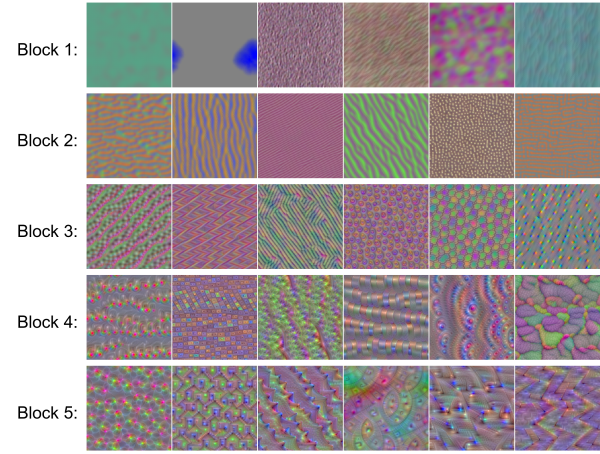
\includegraphics[width=\maxwidth]{/home/susan/Projects/Work/2019-CoNNORFSI/paper/images/labeled_filters} 

}

\caption[Visualizing convolutional filters requires generating images which maximally activate specific filters]{Visualizing convolutional filters requires generating images which maximally activate specific filters. This figure contains images that maximally activate a selection of filters from the convolutional blocks of VGG16. Filters from later blocks detect more complex features than those in earlier blocks. Much like human vision, a hierarchical structure of feature detection with increasing complexity allows CNN ``vision" trained on a general task to be applied to new domains.}\label{fig:vgg16layers}
\end{figure}


\end{knitrout}

In this paper, we demonstrate the use of transfer learning to automatically identify features in shoe treads that are used by forensic examiners. To do this, we leverage the relatively simple structure and generalizability of VGG16 and train a new classifier using a database of labeled shoe tread images we have assembled for this project. This approach differs from other approaches \citep{kongCrossDomainForensicShoeprint2017,kongCrossDomainImageMatching2019a,zhangAdaptingConvolutionalNeural2017} in automatic footwear identification that use the output from the model base directly and do not attempt to add human-friendly contextual information with an additional classifier. The next section describes how the database of images was produced and used to fit our custom classifier.

\paragraph{Annotated Training Data}
Existing research indicates that a sufficiently well-defined set of features can be used to separate shoes into make and model categories \citep{grossVariabilitySignificanceClass2013}; the set of features used in that study included circle/oval, crepe, herringbone, hexagon, parallel lines, logo/lettering/numbering, perimeter lugs, star, and other. After consulting with practitioners, we developed a set of categories suitable for automatic recognition by convolutional neural networks. These modifications were necessary because some of the definitions used in Gross et al. (2013) require contextual spatial information which is not preserved during labeling (for example, lugs are required to be on the perimeter of the shoe). \autoref{tab:class-char-examples} shows three examples of each class in the modified feature set.


The categories we use in this study are operationally defined as follows:
\begin{description}
\item [Bowtie] Bowtie shapes are roughly quadrilateral, with two opposite concave faces. The remaining two faces can be convex or straight, and the concave faces may have straight portions, so long as there is a concave region.
\item [Chevron] Chevron shapes include repeating parallel lines as well as individual ``v" shapes. They may be angular but can also be curved.
\item [Circle] Circles include ellipses and ovals; they must be round.
\item [Line] Lines are repeated and parallel; a more general definition of a line would be difficult to differentiate from many other patterns. Lines can be mildly curved.
\item [Polygon] Polygons are defined in this standard to have more than 4 sides. They include pentagons, hexagons, and octagons.
\item [Quadrilateral] Quadrilaterals (quads) have four sides. They may have rounded or square corners.
\item [Star] Stars are any shape with alternating concave and convex regions, or lines which emanate from a central point. ``X" and ``+" shapes are also classified as stars.
\item [Text] Text is any shape which would be identified as text by a reasonable human. In most cases, the text on the outsole images used is made up of Latin alphabet characters; the model will likely not recognize text in other scripts (but could be trained if non-Latin text images could be obtained).
\item [Triangle] Triangles are any three-sided figure. Like quadrilaterals, they can have rounded corners. In some cases, it is difficult to distinguish between a trapezoidal shape and a triangle when rounded corners are involved.
\item [Other] Other features which were marked include logos, various textures (including crepe, stippling, etc.), and smooth regions with no discernible features. These regions are grouped and provide the additional information that none of the previous nine categories are present.
\end{description}

\begin{table}
\centering
\setlength\tabcolsep{1mm}
\begin{tabular}{rccl}
Bowtie & \raisebox{-.5\height}{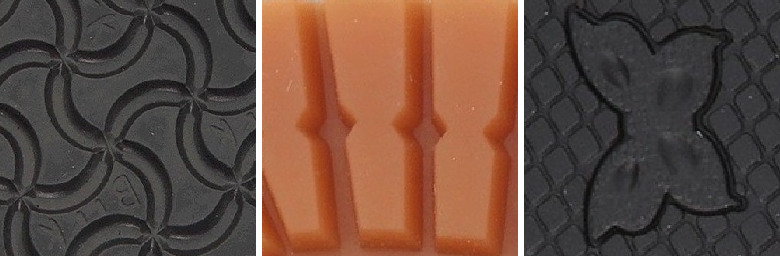
\includegraphics[width=.3\textwidth]{images/class_examples/bowtie_examples.png}} &
\raisebox{-.5\height}{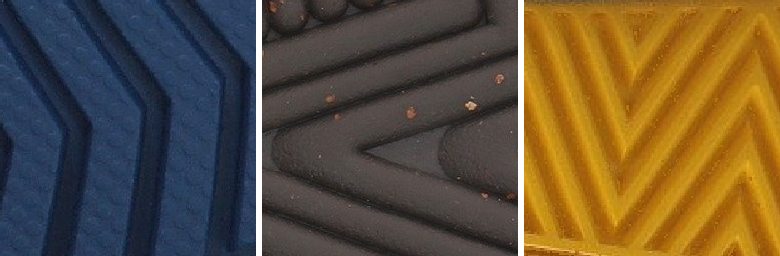
\includegraphics[width=.3\textwidth]{images/class_examples/chevron_examples.png}} & Chevron \vspace{1mm}\\
Circle & \raisebox{-.5\height}{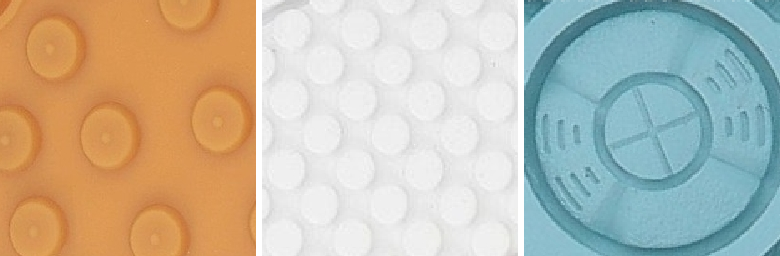
\includegraphics[width=0.3\textwidth]{images/class_examples/circle_examples.png}} &
\raisebox{-.5\height}{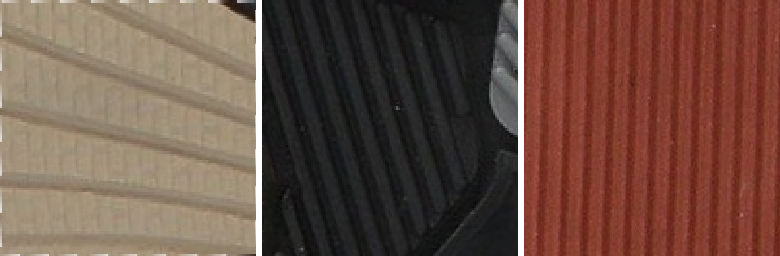
\includegraphics[width=0.3\textwidth]{images/class_examples/line_examples.png}} & Line  \vspace{1mm}\\
Polygon & \raisebox{-.5\height}{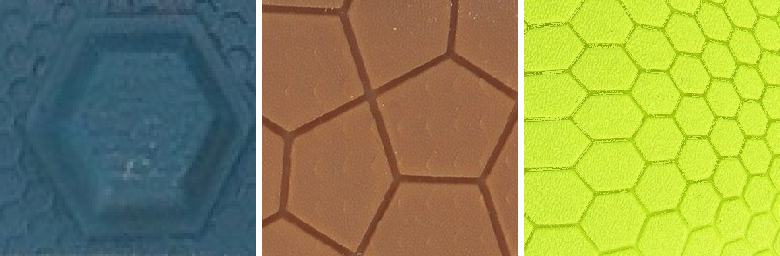
\includegraphics[width=0.3\textwidth]{images/class_examples/polygon_examples.png}} &
\raisebox{-.5\height}{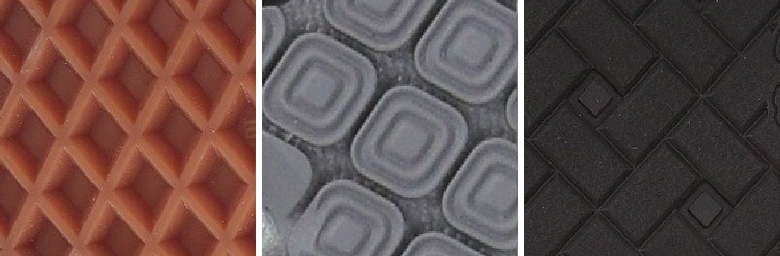
\includegraphics[width=0.3\textwidth]{images/class_examples/quad_examples.png}} & Quad  \vspace{1mm}\\
Star & \raisebox{-.5\height}{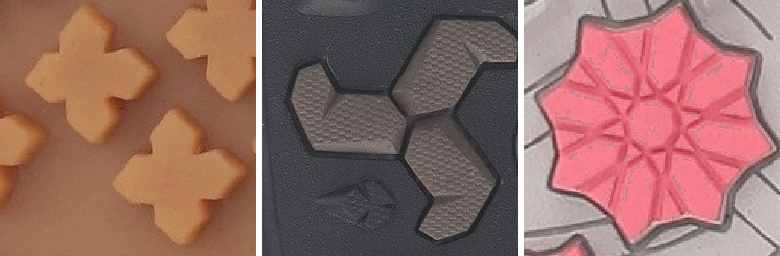
\includegraphics[width=0.3\textwidth]{images/class_examples/star_examples.png}} &
\raisebox{-.5\height}{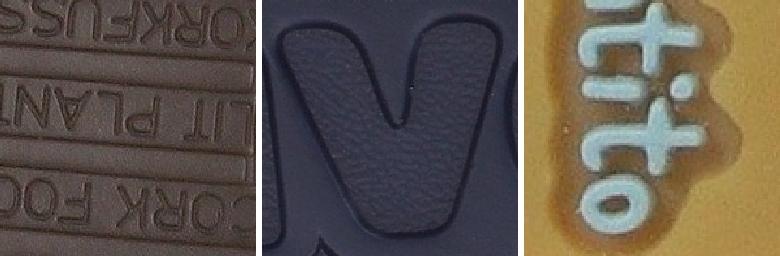
\includegraphics[width=0.3\textwidth]{images/class_examples/text_examples.png}} & Text  \vspace{1mm}\\
Triangle & \raisebox{-.5\height}{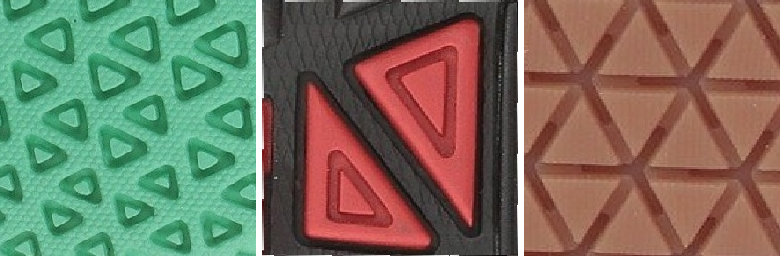
\includegraphics[width=0.3\textwidth]{images/class_examples/triangle_examples.png}} &
\raisebox{-.5\height}{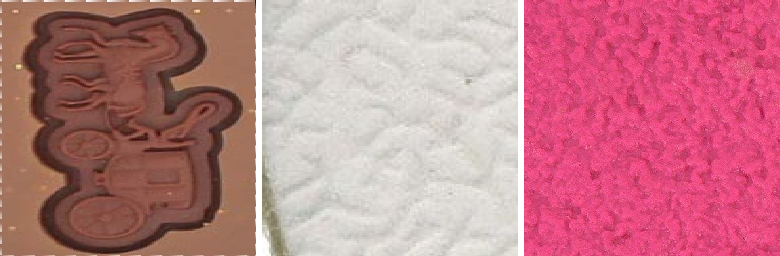
\includegraphics[width=0.3\textwidth]{images/class_examples/other_examples.png}} & Other \\
\end{tabular}
\caption[Geometric elements used to classify tread patterns.]{A set of geometric elements used to classify tread patterns. Categories modified from \cite{grossVariabilitySignificanceClass2013}.}\label{tab:class-char-examples}
\end{table}

Thousands of outsole images were obtained from online shoe retail sites and annotated using LabelMe, a tool for image annotation in computer vision problems \citep{labelme}. After annotation, the minimum bounding rectangle of the region is identified and the image is cropped to that area; subsequently, the cropped image is scaled to 256 x 256 pixels. During this process, aspect ratio is not preserved, though efforts are made to label regions which are relatively square to minimize the effect of this distortion. To date, 4571 shoes have been labeled, yielding 28081 multi-label images.

A reasonable critique of this approach is that images collected from online retailers are of much higher quality than would be expected from the sidewalk scanner proposed in \autoref{sec:Introduction}, and thus the CNN described in this paper is not immediately ready to process real degraded images. This consideration is justified, as machine learning methods tend to perform poorly when applied to test data that do not resemble the training data. However, the use of CNNs to predict class characteristics using the same categories used by human examiners is novel and introduces some interesting complications. As a full-featured automatic scanner is still under development, obtaining representative degraded images is not possible (because the scanner's optics are still in flux). The goal of this work is to evaluate the proposed classification scheme and determine whether CNNs can sufficiently distinguish class characteristic features found on outsoles. Addressing these questions with clean retailer images provides justification for additional algorithm development as well as continuing investment in optimization of the scanner design.


\begin{figure}[hbt]
\centering
\includegraphics[width=.9\textwidth]{images/LabelMe2.png}
\caption{An example of labeling images with LabelMe}
\end{figure}

\begin{knitrout}
\definecolor{shadecolor}{rgb}{0.969, 0.969, 0.969}\color{fgcolor}\begin{figure}

{\centering \includegraphics[width=0.8\linewidth]{figure/class-characteristic-barchart-1} 

}

\caption[Distribution of classes in all labeled images.]{Distribution of classes in all labeled images. Quadrilaterals, lines, circles, text, and chevrons are relatively common; stars, polygons, and bowties are relatively rare.}\label{fig:class-characteristic-barchart}
\end{figure}


\end{knitrout}

Transfer learning reduces the amount of data required to train a CNN by several orders of magnitude, but labeled images are still difficult to generate on a large scale. Thus, to make the most efficient use of the existing labeled data, we enlarge the training data using a process called image augmentation \citep{krizhevskyImageNetClassificationDeep2012}. Augmentation is the transformation of original input data using image operations such as cropping, zoom, skew, rotation, and color balance modification in order to distort or alter the image while maintaining the essential features corresponding to the label. This process reduces the potential for overfitting the model to the specific set of image data used during the training process, and also increases the amount of data available for training. Examples of pre- and post-augmentation images are shown in \autoref{fig:augmented}.

\begin{figure}
\centering
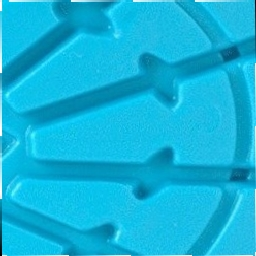
\includegraphics[width=.1\textwidth]{images/augmentation/bowtie_orig.jpg}\hfill

\includegraphics[width=.1\textwidth]{images/augmentation/aug_bowtie.jpg}\hfill\hfill\hfill
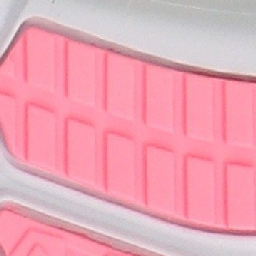
\includegraphics[width=.1\textwidth]{images/augmentation/quad-2_orig.jpg}\hfill
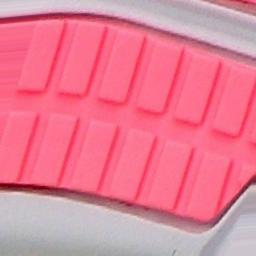
\includegraphics[width=.1\textwidth]{images/augmentation/aug_quad-2.jpg}\hfill\hfill\hfill
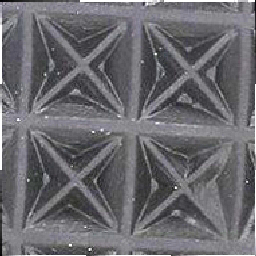
\includegraphics[width=.1\textwidth]{images/augmentation/quad_orig.jpg}\hfill
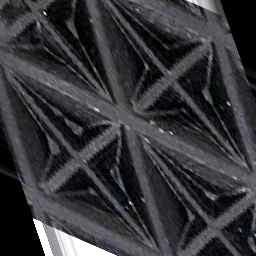
\includegraphics[width=.1\textwidth]{images/augmentation/aug_quad.jpg}\hfill\hfill\hfill
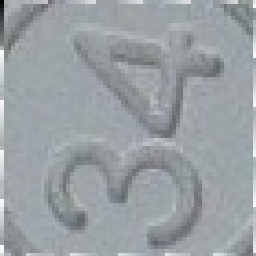
\includegraphics[width=.1\textwidth]{images/augmentation/text_orig.jpg}\hfill
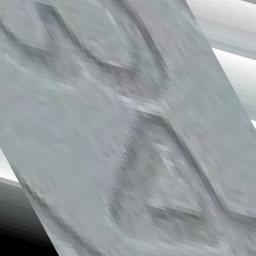
\includegraphics[width=.1\textwidth]{images/augmentation/aug_text.jpg}
\caption[Original and augmented images.]{Four sets of original (left) and augmented (right) labeled images.}\label{fig:augmented}
\end{figure}

Model training is analogous to the human learning process. For example, a child learns to identify dogs by being presented with many labeled examples, such as when their parent uses the label ``dog" for an animal walking by. That child's understanding of dogs is then measured by how many dogs the child is able to correctly identify, and also by the number of other animals it mistakenly calls ``dog". Similarly, CNN training is a series of stages, or ``epochs", where the model learns from the set of labeled training data, and that learning is measured through intermediate predictions on validation data.

The 28081 images were split such that 60\% were used for training. Since the categories do not exist in equal proportion in the labeled data,
the training data were weighted by proportion during the training process to ensure that the model can identify both rare and common geometric shapes. Of the remaining 40\% of data, half were used for validation, to monitor the training process, and the remaining data were for testing the performance of the final model.

\section{Results}

\subsection{Model Training}
During model fitting, the model ``learns" from the training set and is evaluated on the validation set, which consists of previously unseen images (i.e. images not used during the training process). Learning occurs by minimization of the ``loss", which is a function of the distance between the model predictions and the image labels. As the loss decreases, the model's accuracy (the proportion of correct labels) increases. During model training, we expect that the accuracy for the training set will increase beyond the accuracy for the validation set; the validation accuracy will eventually level off. Similarly, we expect the loss for the training set and the validation set to decrease initially. \autoref{fig:training-accuracy} shows the training and validation accuracy and loss at each epoch of the fitting process.

\begin{knitrout}
\definecolor{shadecolor}{rgb}{0.969, 0.969, 0.969}\color{fgcolor}\begin{figure}[h]

{\centering \includegraphics[width=.75\textwidth]{figure/training-accuracy-1} 

}

\caption[Training and validation accuracy and loss during each epoch.]{Training and validation accuracy and loss for each epoch of the fitting process. Training and validation accuracy reach 89.5\% around epoch 9. After that point, validation loss remains the same and training loss decreases slightly, while validation accuracy increases more slowly than training accuracy.}\label{fig:training-accuracy}
\end{figure}


\end{knitrout}

Overfitting occurs when a model learns the training data so well that its understanding of the categories becomes specific to the training cases, which, in turn, leads to poor prediction of new images that were not in the training set. During the training process, overfitting is indicated when the validation loss begins to increase after reaching a global minimum. Alternately, underfitting occurs if the validation accuracy is still increasing when model optimization is terminated (for instance, between epochs 1 and 10 in \autoref{fig:training-accuracy}), because model performance is still improving with continued training. In \autoref{fig:training-accuracy}, validation accuracy levels off after epoch 20, and validation loss has not yet begun to increase at epoch 30, indicating that the model optimization process was halted at an appropriate epoch.

\subsection{Model Accuracy}

\paragraph{Overall Accuracy}
For each image in the test set, the ``true" labels are nine human-assigned labels of 0 or 1 corresponding to the presence or absence of each of the nine shape categories in the image. When the CNN predicts which shapes are in the image, however, it assigns a probability between 0 and 1 for each shape category, with a total of nine probabilities per test image. Thus, to determine the accuracy of the model predictions, we must select a threshold for each label to discretize the model predictions. If the threshold is too low, moderate probabilities will be more likely to exceed the threshold, which increases the true positive and false positive predictions in the test data. Conversely, if the threshold is too high, moderate probabilities will more often fail to meet the threshold, which increases the number of true and false negative predictions. An appropriate threshold must be chosen to produce a high true positive rate while also ideally keeping the false positive rate low. One way to set an optimal threshold is to utilize Receiver Operating Characteristic (ROC) curves, a type of diagnostic plot which compare the false positive rate to the true positive rate for a classification method. \autoref{fig:overall-roc} shows the ROC curve for our model across all classes, and \autoref{fig:class-roc} shows the curve for each class. ROC curves can be summarized by the Area Under the Curve (AUC), which quantifies the overall accuracy of the model. Perfect prediction would be indicated by a right angle along the upper left corner of the plot, with a corresponding AUC of 1, and a diagonal line with an AUC of 0.5 would indicate that the classification method performs no better than random chance.

\begin{knitrout}
\definecolor{shadecolor}{rgb}{0.969, 0.969, 0.969}\color{fgcolor}\begin{figure}

{\centering \includegraphics[width=.5\textwidth]{figure/overall-roc-1} 

}

\caption[Overall model performance ROC curve.]{ROC curve showing overall model performance. Model accuracy is generally high, as the ROC curve is significantly above the identity line $y=x$.}\label{fig:overall-roc}
\end{figure}


\end{knitrout}

\begin{knitrout}
\definecolor{shadecolor}{rgb}{0.969, 0.969, 0.969}\color{fgcolor}\begin{figure}

{\centering \includegraphics[width=\textwidth]{figure/class-roc-1} 

}

\caption[Class-by-class ROC curves.]{Class-by-class ROC curves. AUC is area under the curve, a measure of overall model performance. Equal error rates (EER) are marked, indicating the position at which there is equal probability of a false positive or false negative error.}\label{fig:class-roc}
\end{figure}


\end{knitrout}

The full model has an AUC of 0.88, and the AUC for individual classes ranges from 0.81 (for line) to 0.93  (for bowtie).
While the class performances do vary slightly, each ROC curve indicates that the model performs significantly better than random chance. The points in \autoref{fig:class-roc} represent the equal error rate (EER), which is the threshold where there is equal probability of a false positive or false negative error. We will use a class specific EER to set an individual threshold for each class, so that any model prediction with probability above the EER for that shape is considered a positive prediction.

\paragraph{Class Accuracy}
The ROC curves provide only a general summary of model accuracy; to learn more about how specific images are classified, we can view images from the test set along with the nine class predictions assigned by the model. \autoref{fig:exemplars} and \autoref{fig:circle-text-consistency} show model predictions for a selection of images. Each image shown in the following examples belongs to either the validation or test data, so none of the images were used during model training. In these figures, the values in each row are the predicted probabilities for the nine classes in the corresponding image, such that each column represents predictions for a given class. The saturation of blue color corresponds to the strength of the predicted probability, and the navy blue border around an image indicates that the predicted probability is above the EER threshold for the given class. Note that the EER is not the same for all classes; in other words, the same probability value assigned across different categories may yield different conclusions about whether the model predicts the shape is present or absent in the image.

The first rows of \autoref{fig:exemplars} are images which contain only one of the nine classes. Most of the predictions for these images are promising; there are some false-positive labels that indicate confusions between circle/text and polygon/quad, but all of the true shapes are correctly identified by the model above their respective EER. The next image belongs to the ``other" category, as it does not contain any of the nine classes; the model correctly assigns near-zero probabilities to each class. The final rows are of images that belong to more than one class category. Again, predictions are largely accurate, with most of the prominent shapes correctly identified above EER. The most notable misclassifications in these images are the false positive predictions of triangle in the image with green text and lines in the Adidas logo. Although the Adidas logo is technically made up of adjacent quadrilaterals, the prediction of a triangle is reasonable when considering the proximity of those quadrilaterals and the shape's features as a whole, and the relatively low predicted probability suggests that the model recognizes that this shape is ambiguous. All other predictions for these images are accurate given our operational definition of class categories.



\begin{knitrout}
\definecolor{shadecolor}{rgb}{0.969, 0.969, 0.969}\color{fgcolor}\begin{figure}[p!]

{\centering \includegraphics[width=1\linewidth]{figure/exemplars-1} 

}

\caption[Model predictions of images containing (from the top) a single shape, no shape, or multiple shapes across all categories]{Model predictions of images containing (from the top) a single shape, no shape, or multiple shapes across all categories. Predicted probabilities greater than the equal error rate threshold are outlined in blue. Although there are some misclassifications, predictions are generally consistent with the human-assigned labels of these images.}\label{fig:exemplars}
\end{figure}


\end{knitrout}

While figure \ref{fig:exemplars} shows representative examples of classifications across multiple shape categories, it is also useful to examine many cases within a given shape to get a sense of model consistency. \autoref{fig:circle-text-consistency} shows a number of images containing circles and/or text. The top four rows show text contained within a separate, distinct circle shape, and the next five rows show circles represented as the letter ``o" in text. The remaining images contain only one of either text or circles, as well as other possible shape categories. In particular, the first two of these images contain text that use the capital letter ``G", the next two images contain no circular shapes, and the final 3 images contain pure circles that do not appear to belong to text. The model is able to identify the circle in all cases where a circle is truly present, regardless of whether the circle is part of the text or it is distinct; however, the circle prediction is also strong in three of the four images that do not contain a circle, which indicates that the model is having difficulty distinguishing the two categories. While the circle predictions are often above the EER for letters such as G and S, these predictions are generally much lower than those where distinct circles or Os are seen, indicating that there are some indications that features are not as strong in the quasi-circle shapes, but that the model is not able to completely separate Os from C, S, and G shapes which are also very circular. This confusion is complicated by the frequency of images which contain both circles and text: text is present in 39\% of our labeled images containing circles, and circles are present in 31\% of our images containing text. In addition, the distinction between a circle and an ``o" comes from the context around the shape, which is much more difficult for the model to parse than simply detecting a shape. More importantly, this behavior does not suggest poor model performance as much as a weakness of the classification scheme, which will be discussed in a later section.

\begin{knitrout}
\definecolor{shadecolor}{rgb}{0.969, 0.969, 0.969}\color{fgcolor}\begin{figure}[p!]

{\centering \includegraphics[width=1\linewidth]{figure/circle-text-consistency-1} 

}

\caption[Model predictions of images containing circles and/or text]{Model predictions of images containing circles and/or text. The model correctly identifies circles in all images where circles are present, but also predicts moderate probabilities of circles in many images where text is present with curved letters, such as ``G". Text is correctly identified in most images, with the exception of the false negative prediction of the low-contrast text within a hexagon and the false positive prediction of concentric circles.}\label{fig:circle-text-consistency}
\end{figure}


\end{knitrout}

% \paragraph{Confusion Matrix}
Figures \ref{fig:exemplars} and \ref{fig:circle-text-consistency} show predictions for a number of individual images. Many of the misclassifications in these examples, however, are not just seen in individual images, but rather exist systematically between certain classes. A confusion matrix is a type of visualization that summarizes the relationships between the labels assigned to an image and the labels predicted by the model across all test data, and is a helpful diagnostic tool to understand which classes are systematically misclassified. The confusion matrix for the fitted model is presented in \autoref{fig:confusion-matrix}. The values along the diagonal of the matrix represent the proportion of true positives captured within each category. The off-diagonal values represent the proportion of false positives for each shape pairing; however, since a single image may truly contain multiple shapes, the values have been adjusted to remove the effect of any true positives from the calculation of false positive proportions. Thus, this might be considered a conditional confusion matrix, because we condition the off diagonal probabilities on the label not being correct. For example, to calculate the proportion of images that contain triangles but are being falsely labeled as containing quadrilaterals, any images that truly contains both triangles and quadrilaterals are removed before calculating the proportion of false quadrilateral labels. As a result of this adjustment, the off-diagonal values of the confusion matrix are the proportion of images within a true class (column-wise) that are falsely labeled as containing another class that has not been labeled in the image (row-wise). Note that this matrix is not symmetric: the proportion of images containing text that are falsely predicted to contain circles is not necessarily equal to the proportion of images containing circles that are falsely predicted to contain text.

\begin{knitrout}
\definecolor{shadecolor}{rgb}{0.969, 0.969, 0.969}\color{fgcolor}\begin{figure}

{\centering \includegraphics[width=\textwidth]{figure/confusion-matrix-1} 

}

\caption[Confusion matrix, with correct and incorrect model classifications.]{Confusion matrix, showing on the diagonal the correct classification rate and on the off-diagonal, classification errors. Note that in multi-label images, correct off-diagonal labels have been excluded from the calculation of false positives. Quadrilaterals are generally over-predicted across true labels; polygons and triangles are under-predicted. Circles and text are also often confused.}\label{fig:confusion-matrix}
\end{figure}


\end{knitrout}

The horizontal band in \autoref{fig:confusion-matrix} indicates that quadrilaterals are predicted more often than they should be for every true label. Similarly, polygons and triangles produce a moderate number of false positive predictions in other categories, as evidenced by the vertical bands for these categories. It is also apparent that circles and text are commonly confused, which supports our earlier observations from \autoref{fig:circle-text-consistency} that these two classes are difficult for the model to distinguish, in part because circles are relatively common components of Latin script characters.

\subsection{Model Diagnostics}
After examining model performance, both in specific cases and systematically across classes, there seem to be two primary reasons for misclassifications: poor image contrast, and overlapping features between categories.

\paragraph{Image Contrast}
As described earlier, the images used for this research were obtained from online retailers before being labeled and cropped. One consequence of using outsole images instead of impressions is the impact of colors in the image. Features from outsoles that are primarily black or white in color are typically not as prominent as features from images with more varied color schemes. As a result, the features in low contrast images are not easily resolved by the filters; this is propagated through both model training and prediction of new images. In other words, the model `learns' that when there are few meaningful features with which to determine which shapes are present, the best strategy for minimizing loss is to predict diffuse probabilities across many classes, as seen in \autoref{fig:low-contrast-consistency}.

\begin{knitrout}
\definecolor{shadecolor}{rgb}{0.969, 0.969, 0.969}\color{fgcolor}\begin{figure}[p!]

{\centering \includegraphics[width=1\linewidth]{figure/low-contrast-consistency-1} 

}

\caption[Model predictions for images with low contrast]{Model predictions for images with low contrast. While these images contain a variety of shapes (as shown in the color-corrected column on the right), the diffuse probabilities assigned by the model across all categories indicate that features are obscured by low contrast, which propogates through model training and prediction.}\label{fig:low-contrast-consistency}
\end{figure}


\end{knitrout}

\paragraph{Feature Overlap}
We have defined our categories through consultation with practitioners and modifications of previous research, but as a result, there are a number of features (such as lines, angles, and curves) which are not unique to only one category. For example:
\begin{itemize}
\item a triangle may be made up of three acute angles, but a quadrilateral can also contain three acute angles.
\item the only distinction between an ``o" and a circle is whether there is more text around it.
\item the only difference between lines and thin repeating quads are the ends of the shapes.
\end{itemize}

To detect these shapes, the model is doing a significant amount of feature integration beyond just detecting the presence of raw lines, angles, and curves. A correct classification requires the detection and integration of (often) relatively large features (with respect to filters only a few pixels wide); in addition, features can be relatively small relative to the 256x256 image, or may take up the entire image. This wide variation in relative size of the features, combined with the variability of different features across classes, leads to a number of common (but understandable) misclassifications.

This is one area where the CNN's predictions do not match human labels; in part, this is because even with some wider context, the CNN does not use both bottom-up feature integration and top-down object identification based on wider experience - as a result, it cannot easily differentiate between text and constituent shapes within the text.

This issue is exacerbated by the variability of images within a class. A quadrilateral isn't just a square or rectangle with 4 right angles; it can also be a parallelogram, diamond, trapezoid, part of a chevron, or anything else that has four sides. In general, some of our identified shapes are very common on outsoles and appear in our data in many different forms, which further widens the sets of features the model must learn to associate with a single class. Unfortunately, by associating even more possible features with a single category, the number of features that then overlap between categories also increases.

The shape categories with the largest number of images, shown in \autoref{fig:class-characteristic-barchart}, also tend to have the most variability in labeled images. This is supported by \autoref{fig:brand-plots}, which breaks down, by proportion, the top ten most frequent brands in the labeled data for each class. The figure shows that, for example, a relatively large proportion of bowties in our labeled data are contributed by images of Birkenstocks. Since the bowties on Birkenstocks tend to be similar in shape and size, the model is able to create a relatively stable definition of bowties and thus predicts new images of bowties well. There is no similar consistency in categories like quadrilaterals. \autoref{fig:brand-plots} indicates that no one brand makes up more than 4\% of our labeled quadrilateral images. This suggests that the quadrilaterals in our labeled data are more likely to come in a variety of shapes and sizes, so it is more difficult for the model to learn which set or sets of features correspond to a quadrilateral.

\begin{knitrout}
\definecolor{shadecolor}{rgb}{0.969, 0.969, 0.969}\color{fgcolor}\begin{figure}

{\centering \includegraphics[width=1\linewidth]{figure/brand-plots-1} 

}

\caption[Proportions of top 10 shoe brands in our labeled dataset within each shape category, sorted by prevalence]{Proportions of top 10 shoe brands in our labeled dataset within each shape category, sorted by prevalence. Brand text is present when the brand makes up more than five percent of labeled shoes for the shape category. Some shapes, like bowtie and polygon, are relatively dominated by a small number of brands while other shapes, such as text and quad, are comprised of a large number of brands. Typically, model predictions are best for shape categories without much variability, which, in general, coincides with shapes dominated by a small number of brands.}\label{fig:brand-plots}
\end{figure}


\end{knitrout}

We have proposed several hypotheses to explain the inconsistencies between the manual labels and the model's predictions on the images. We can test these hypotheses by examining what the model ``sees" when making its predictions. Heatmaps, also known as Class Activation Maps (CAMs), are a visual diagnostic tool that highlights the areas of an image that are most significant to classification for a given class \citep{chollet_allaire_2018}. Using these graphics, we can identify which locations in an image contribute most to the model's predictions.

Figures \ref{fig:ugg-heatmap}-\ref{fig:dc-heatmap} show a number of images alongside heatmaps for the four classes with the highest output probabilities for each image. \autoref{fig:ugg-heatmap} shows predictions and heatmaps for the logo from an UGG shoe. The model correctly identifies triangles and text, and references appropriate regions of the image. The prediction of a circle is shown to be associated with the letter ``G"; although this prediction is technically incorrect, it indicates that the model has learned to associate curved shapes with circles. This association is again seen in the high predicted probability of circle in \autoref{fig:seychelles-heatmap}. In this case, the prediction of text is again correct,, but the prediction of circle is not---there are very round shapes, but they do not form a closed figure that could be identified as a circle. \autoref{fig:dc-heatmap} shows a DC shoe with repeating instances of a shape that is a combination of a circle and quadrilateral, but does not technically fall into either of those categories by our definition. The model assigns high probabilities of circle and quadrilateral and indicates that the proper image features are being used for this classification. Additionally, the prediction of polygon is incorrect but reasonable considering that many small hexagons are indistinguishable from circles. These heatmaps can confirm that a number of misclassifications are a result of overlapping features between classes, and that the model is using reasonable features to make predictions.



\begin{knitrout}
\definecolor{shadecolor}{rgb}{0.969, 0.969, 0.969}\color{fgcolor}\begin{figure}[!p]

{\centering 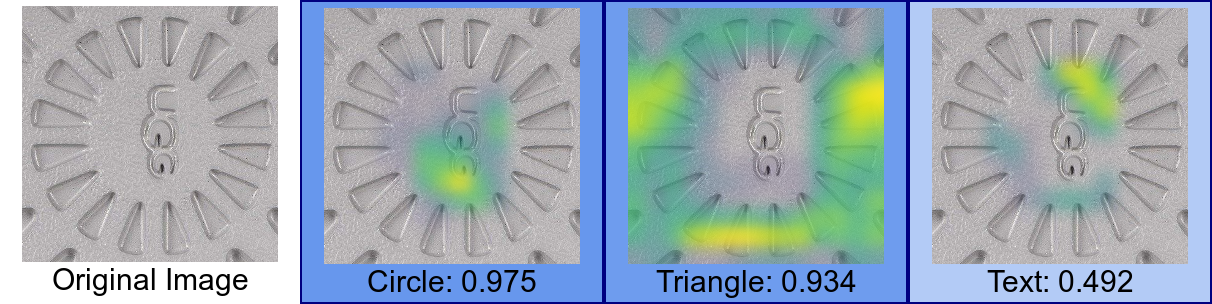
\includegraphics[width=.95\textwidth]{/home/susan/Projects/Work/2019-CoNNORFSI/paper/images/heatmaps/processed/heatmap-a7-Ugg-grey} 

}

\caption{A section of an UGG shoe containing the logo. The model correctly identifies triangles and text (and references the correct portion of the image in both cases). The model identifies a circle as well; while it could be argued that the triangles form an implicit circle, the heatmap demonstrates that the circular portion of the image is the ``G", which would not be a closed figure labeled as a circle. The model's prediction of the presence of a circle is understandable, but incorrect.\label{fig:ugg-heatmap}}\label{fig:current-heatmaps1}
\end{figure}

\begin{figure}[!p]

{\centering 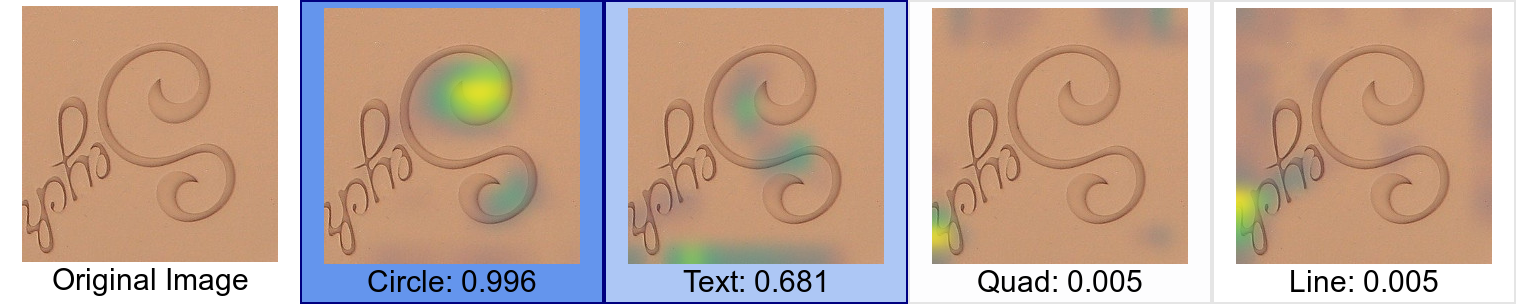
\includegraphics[width=.95\textwidth]{/home/susan/Projects/Work/2019-CoNNORFSI/paper/images/heatmaps/processed/heatmap-text-seychelles} 

}

\caption{In this image of a Seychelles shoe, the model identifies text and circle. The prediction of text is correct; the prediction of circle is not---there are very round shapes, but they do not form a closed figure that could be identified as a circle.\label{fig:seychelles-heatmap}}\label{fig:current-heatmaps2}
\end{figure}

\begin{figure}[!p]

{\centering 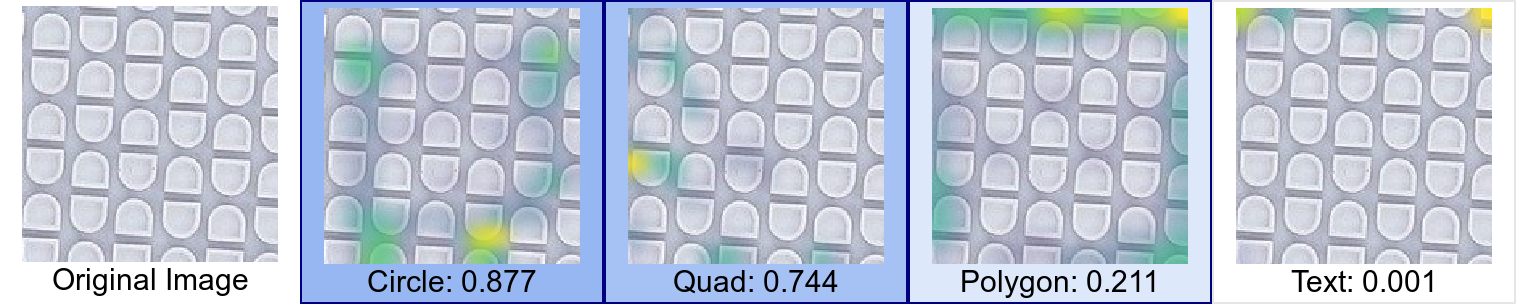
\includegraphics[width=.95\textwidth]{/home/susan/Projects/Work/2019-CoNNORFSI/paper/images/heatmaps/processed/heatmap-04-circle_quad-2-dc-vestrey-black-camo_product_9065558_color_12784} 

}

\caption{This image from a DC shoe contains repeating instances of a shape that appears to be a combination of a circle and quadrilateral, but does not technically fall into any of the nine categories used in our labeling scheme. The model assigns high probabilities of circle and quadrilateral and indicates that the proper image features are being used for this classification. The prediction of polygon is incorrect but reasonable considering that many small hexagons are indistinguishable from circles.\label{fig:dc-heatmap}}\label{fig:current-heatmaps3}
\end{figure}


\end{knitrout}












\section{Conclusions}
% Restate goal and briefly summarize methods

In this paper, we have presented a method for automatic identification of geometric class characteristics in outsole tread patterns. A set of geometric class characteristics were defined based on feature sets currently used by examiners and used to classify a large variety of tread patterns. Labeling these images provided the opportunity to select a manageable number of features and define criteria for labeling these features on newly collected footwear images. Using the convolutional base of VGG16, a pre-trained neural network, we created a new classifier optimized to work with outsole images. This classifier returns the probability of each geometric feature for new outsole images.

% Discussion of weaknesses
Although model predictions are generally accurate, there are a number of systematic misclassifications and weaknesses which can be addressed in future iterations of the modeling process. The model has substantial difficulty predicting images with low contrast because image features are obscured. Exploring methods of color correction, such as histogram equalization, may prove useful for eliminating the effect of contrast on predictions. Initial implementations of histogram equalization suggest that the overall accuracy improvement is modest; the model fit to images which have been equalized had approximately 92.5\% validation accuracy, an improvement of 1.5\% over the default model described in this paper.

Another source of systematic misclassifications stems from the inherent overlap between features of common geometric shapes. CNNs make predictions via bottom-up feature integration; as a result, it is more difficult for the model to distinguish between geometrically similar shapes, such as chevrons and triangles. This issue is exacerbated by high variability of some shapes commonly found in outsole patterns, which requires the model to form a flexible understanding of each shape category and makes distinction between similar shapes even more difficult. These issues of overlap and variability are at least in part due to our decision to use the features used by practitioners directly; some of this may also result from our operational definitions of various shapes, which were created before we had a complete understanding of the practical limitations of CNNs. While a complete remedy may not be possible, there may be some modifications to operational class definitions that we can make to optimize labels for model prediction. In addition, we will continue to improve the labeling of shapes in our database with the goal of expanding the breadth and quantity of labeled images available for model training.

Although there are many areas for potential improvement in future iterations of this model, we have demonstrated the effectiveness of using transfer learning to provide an initial label for shoe outsole patterns. As most of the misclassifications are systematic, it is clear that the model is able to learn features and apply rules consistently. We expect that the proposed modifications to the labeling criteria and data processing pipeline will improve the model's accuracy, but the 91\% validation accuracy is promising considering that we do not have estimates of the consistency of examiners' estimates on ambiguous features. Taken together, these factors show that Convolutional Neural Networks are a useful tool for classifying a large number of outsoles within a common classification scheme, although further research is needed into designing human comphrehensible classification schemes for this purpose. This work thus provides the necessary proof-of-concept that a well-trained model within an appropriate classification scheme, in conjunction with images collected from a footwear scanner, can be used to estimate the coincidental match probability of footwear tread patterns.





\bibliography{mybibfile}

\end{document}
